\documentclass{article}

% 312 Font
\usepackage{charter}
% Custom lists
\usepackage{enumitem}
% Page margins & pagestyles
\usepackage{fullpage}
% Font encoding
\usepackage[T1]{fontenc}
% Colored boxes around the 'solution' environment
\usepackage{mdframed}
% Used for making FSMs
\usepackage{tikz}
\usetikzlibrary{automata}
% For color
\usepackage[dvipsnames]{xcolor}

% Defines a solution environment that creates a green box around text inside.
\mdfdefinestyle{SolutionFrame}{linecolor=green!60!black,linewidth=1pt}
\newenvironment{solution}{\begin{mdframed}[style=SolutionFrame]}{\end{mdframed}}

% Enumerate with (a),(b),(c),...
\newenvironment{enum}{\begin{enumerate}[label={(\alph*)}]}{\end{enumerate}}

% Put a dot after section titles
\renewcommand\thesection{\arabic{section}.}
\renewcommand\thesubsection{\arabic{section}.\arabic{subsection}.}

% Tikz styles & configs
\tikzset{
    ->,
    node distance=2cm,
    initial text=$ $,
}

% Images {img_size = 1.0, file_path}
\newcommand{\img}[2][1.0]{
    \begin{minipage}[t]{0.9\linewidth}
        \begin{center}
            \includegraphics[width=#1\linewidth]{#2}
        \end{center}
    \end{minipage}
}

% Hide the Date
\date{}
% Hide page numbers
\pagenumbering{gobble}

\begin{document}
    \begin{titlepage}
        \centering
        \null
        \vspace{5cm}
        {\Huge CSE 369 Lab 7\par}
        \vspace{0.5cm}
        {\Large Useful Components \par}
        \vfill
        {\hfill \Large Isaac Wu \par}
        {\hfill \large 2360957 \par}
        {\hfill \large \today \par}
    \end{titlepage}

\section{Top-Level Block Diagram}
    \begin{solution}
        \img[1.1]{block_diagram.png} \\
        
        This is my Top-Level Block Diagram for the Cyber War module. The Cyber War module takes in 12 inputs, KEY0 (for Player Input), KEY3 (to reset the playfield after a victory), SW9 (to reset the game), and SW8-0 (to calibrate the difficulty of the cyber player). Only the player input needs to be synchronized, so it gets passed through two D-flip-flops to account for metastability. I then pass in the user input into an Edge Detector to reduce each button press to one cycle in length since our clock is very fast.
        
        A 9-Bit LFSR is initialized and its status is read as an unsigned number. The current state of the LFSR is added with the unsigned number interpreted from SW8-0. If the resulting sum is above a certain threshold, then the cyber player will input on the next clock edge.
        
        The inputs for both players, along with the reset and soft reset inputs are all passed into each of the 9 light modules. These light modules have their own state and will determine whether or not their linked LED will be lit, which is output to the LEDRs outside of the top level module.
        
        The status of the lights on each edge are passed in along with the players' inputs and the reset input to two counter modules, one to keep track of each player's win count. These counters are responsible for updating their linked HEX display (HEX5 for the cyber player and HEX0 for the player) when their corresponding player has won.
    \end{solution}

\newpage
\section{3-Bit Counter Simulation}
    \begin{solution}
        These are the resulting waves of a test bench to verify functionality of my 3-bit counter. The last combined wave is the binary output assigned to HEX display modules that have been predefined to display the numbers 0-7. The input is toggling after each rising clock edge, and each toggle on increments the counter at the next rising clock edge, and reset inputs will revert the output to the defined binary for 0. \\
        \img[1.1]{counter_waves.png}
    \end{solution}

\section {4-Bit LFSR State Diagram}
    \begin{solution}
        This is the state diagram for a 4-Bit Linear Feedback Shift Register. The next state is determined by shifting the 3 least significant bits to the 3 most significant bits and setting the least significant bit to the XNOR of the two most significant bits. In the diagram, the arrows with a * represent that the transition will always be taken. Note that the 1111 state is separate from the diagram and can only lead to itself.
        \begin{center}
        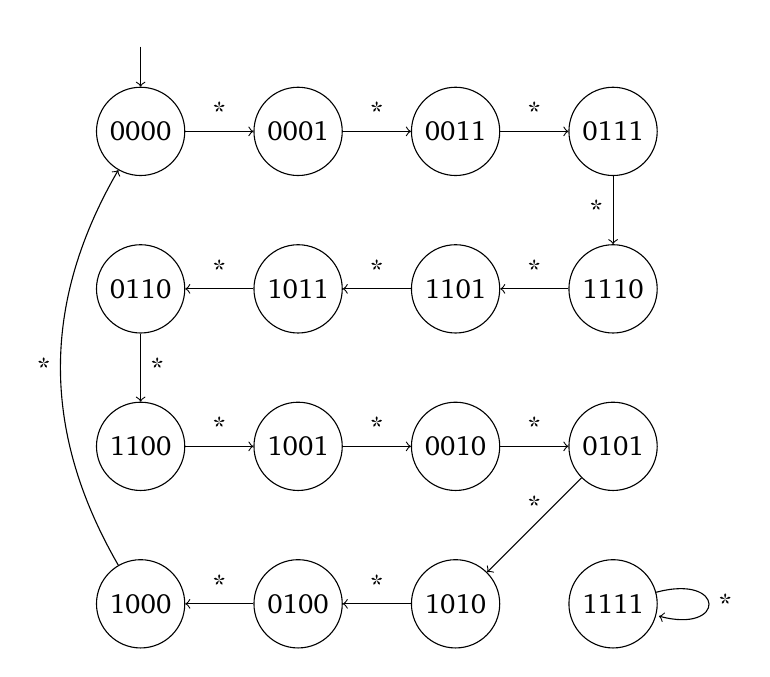
\begin{tikzpicture}
            \node[state, initial, initial where=above] (0000) {0000};
            \node[state, right of=0000] (0001) {0001};
            \node[state, right of=0001] (0011) {0011};
            \node[state, right of=0011] (0111) {0111};
            \node[state, below of=0111] (1110) {1110};
            \node[state, left  of=1110] (1101) {1101};
            \node[state, left  of=1101] (1011) {1011};
            \node[state, left  of=1011] (0110) {0110};
            \node[state, below of=0110] (1100) {1100};
            \node[state, right of=1100] (1001) {1001};
            \node[state, right of=1001] (0010) {0010};
            \node[state, right of=0010] (0101) {0101};
            \node[state, below of=0101] (1111) {1111};
            \node[state, left  of=1111] (1010) {1010};
            \node[state, left  of=1010] (0100) {0100};
            \node[state, left  of=0100] (1000) {1000};

            \path
                (0000) edge node[above] {*} (0001)
                (0001) edge node[above] {*} (0011)
                (0011) edge node[above] {*} (0111)
                (0111) edge node[left]  {*} (1110)
                (1110) edge node[above] {*} (1101)
                (1101) edge node[above] {*} (1011)
                (1011) edge node[above] {*} (0110)
                (0110) edge node[right] {*} (1100)
                (1100) edge node[above] {*} (1001)
                (1001) edge node[above] {*} (0010)
                (0010) edge node[above] {*} (0101)
                (0101) edge node[above] {*} (1010)
                (1010) edge node[above] {*} (0100)
                (0100) edge node[above] {*} (1000)
                (1000) edge[bend left] node[left] {*} (0000)

                (1111) edge[loop right] node[right] {*} (1111)
            ;
        \end{tikzpicture}
        \end{center}
    \end{solution}

\newpage
\section{9-Bit LFSR Simulation}
    \begin{solution}
        The beginning of my LFSR simulation. You can see that i is counting the number of states after the initial state, for which I have an indicator signal set to be true only when the out state is 0, and these change every rising clock edge. \\
        \img[1.1]{lfsr_start.png}
        \clearpage
        This diagram shows the next edge that my indicator is signal is true and the out state is once again 0. Here, it shows that i is now 511, indicating to us that the maximum state cycle length is 511 states. \\
        \img[1.1]{lfsr_end.png}
    \end{solution}

\newpage
\section{10-Bit Adder Simulation}
    \begin{solution}
        The top 3 waves are unsigned, the bottom 3 are the same values, just signed. \\
        \img{adder_waves.png}
        \begin{enumerate}[label=\arabic*)]
            \item An addition with one input being 0: 0 + 1 = 0
            \item An addition whose result is 511: 369 + 142 = 511
            \item An addition whose result is 0: 369 + -369 = 0
            \item An example of unsigned overflow: 369 + 655 = 0, 1023 + 1023 = 1022
            \item An example of positive signed overflow: 511 + 511 = -2
            \item An example of negative signed overflow: -512 + -512 = 0
        \end{enumerate}
    \end{solution}

\newpage
\section{Top-Level ModelSim Simulation}
    \begin{solution}
        As a reminder, SW[9] represents a hard reset (resets the game), KEY[3] represents a soft reset (resets the playing field), KEY[0] is the user input, SW[8-0] represents the difficulty of the Cyber player, and L is the Cyber player ``input''. \\~\\
        This is the wave diagram for the initial state of Cyber War, right after a reset input. In this scenario, I set the Cyber player's difficulty to 512/1023. LED 5 is on, the rest are inactive. Both HEX displays are showing the pre-defined binary to display a 0. \\
        \img{war_init.png} \\
        This is what a wave diagram of the Cyber player winning looks like. The Cyber player pseudo-randomly ``presses'' an input and the LED status light moves to the left at the next clock cycle after each input (since we don't have to synchronize the Cyber player's inputs). After the status light moves off of the final LED position, the HEX display for the cyber player will increment to the pre-defined binary to display a 1. Inputs after a win don't change the LED output or the HEX output. \\
        \img{cyber_win.png}
        \newpage
        This is a wave diagram of Player winning. The same thing happens, just in reverse. The Cyber player has been slowed down to 1/1023, and does not make an input in this sequence. The LED status light starts in the center and moves to the right. After it falls off the right, the HEX display for the player will change to display a 1. Again, any inputs after a victory will not change any displays. A soft reset input will reset the LEDs, but notice the HEX displays retain their previous values. \\
        \img{player_win_1.png} \\
        \img{player_win_2.png}
    \end{solution}

\section{Resource Utilization}
    \begin{solution}
        \img{resources.png}
    \end{solution}

\section{Misc.}
    How many hours (estimated) it took to complete this lab in total, including reading, planning, designing, coding, debugging, and testing.
    \begin{solution}
        It took around 10 hours to complete this lab.
    \end{solution}

\end{document}